\documentclass[11pt,a4paper]{article}
\usepackage{gtu-el-yazisi}
\begin{document}
\notbilgi{İşaretler ve Sistemler}{Ders 6 -- Sürekli zamanlı Fourier serisinin özellikleri}{Isaret-ve-Sistemler-ders-6.pdf}
\renewcommand{\thempfootnote}{\alph{mpfootnote}} % kutu içi dipnotlar için (euler + \itshape uyumsuzluğu)

\section{Sürekli zamanlı Fourier serisinin özellikleri}
\sayfa{1}
\[ x(t) = x(t + T_0), \qquad \omega_0 = 2\pi f_0 = \frac{2\pi}{T_0} \]
\[ x(t) \xleftrightarrow{\ FS\ } x_k \]

\subsection{1) Scalar multiplication:}
\[ \alpha\,x(t) \xleftrightarrow{\ FS\ } \alpha\,x_k \]

\subsection{2) Lineerlik:}
\[ \alpha\,x_1(t) + \beta\,x_2(t) \xleftrightarrow{\ FS\ } \alpha\,x_{1,k} + \beta\,x_{2,k} \]
$x_1(t)$ ve $x_2(t)$'nin periyodu ($T_0$) / frekansları ($\omega_0$) aynı olmalıdır.

$\alpha\,x_1(t) + \beta\,x_2(t)$ işaretinin periyodu da $T_0$'dır.

\subsection{3) Zamanda tersini alma (time reversal):}
\[ x(-t) \xleftrightarrow{\ FS\ } x_{-k} \]
$\Rightarrow$ $x(t)$ çift işaret ise FS katsayıları da çifttir.
\[ x(t) = x(-t) \xleftrightarrow{\ FS\ } x_k = x_{-k} \]
$\Rightarrow$ $x(t)$ tek işaret ise FS katsayıları da tektir.
\[ x(t) = -x(-t) \xleftrightarrow{\ FS\ } x_k = -x_{-k} \]

\subsection{4) Zamanda öteleme:}
\[ x(t - t_0) \xleftrightarrow{\ FS\ } x_k\,e^{-jk\omega_0 t_0} \]
İspat: \ $x(t - t_0) \xleftrightarrow{\ FS\ } d_k$ olsun
\[ d_k = \frac{1}{T_0}\int_{T_0} x(t - t_0)\,e^{-jk\omega_0 t}\,dt \underset{\substack{\uparrow\\ t - t_0\,=\,\tau}}{=} \frac{1}{T_0}\int_{T_0} x(\tau)\,e^{-jk\omega_0(\tau + t_0)}\,d\tau = e^{-jk\omega_0 t_0}\underbrace{\frac{1}{T_0}\int_{T_0} x(\tau)\,e^{-jk\omega_0\tau}\,d\tau}_{=\,x_k} \]
\[ d_k = x_k\,e^{-jk\omega_0 t_0} \]
$|d_k| = |x_k| \longrightarrow$ Periyodik bir işaretin zamanda ötelenmesi FS katsayılarının genliğini değiştirmez.

\subsection{5) Frekansta öteleme:}
\[ x(t)\,e^{jk_0\omega_0 t} \xleftrightarrow{\ FS\ } x_{k-k_0} \]
İspat: \ $d_k = \dfrac{1}{T_0}\displaystyle\int_{T_0} x(t)\,e^{jk_0\omega_0 t}\cdot e^{-jk\omega_0 t}\,dt = \dfrac{1}{T_0}\displaystyle\int_{T_0} x(t)\,e^{-j(k - k_0)\omega_0 t}\,dt = x_{k-k_0}$

\subsection{6) Zamanda ölçeklendirme:}
\[ x(\alpha t) \xleftrightarrow{\ FS\ } x_k \]
Periyodik bir işaretin zamanda ölçeklendirilmesi FS katsayılarını değiştirmez. Ancak, $x(\alpha t)$ işaretinin frekansı $\alpha\omega_0$ ve periyodu $\dfrac{T_0}{\alpha}$ olarak değişir.

\subsection{7) Çarpma:}
(Frekansta konvolüsyon)
\[ x_1(t)\cdot x_2(t) \xleftrightarrow{\ FS\ } x_{1,k} \ast x_{2,k} = \sum_{n=-\infty}^{\infty} x_{1,n}\,x_{2,k-n} \]

\subsection{8) Zamanda türev alma:}
\[ \frac{d^n x(t)}{dt^n} \xleftrightarrow{\ FS\ } (jk\omega_0)^n\,x_k \]

\subsection{9) Eşlenik alma (conjugation):}
\[ x^{*}(t) \xleftrightarrow{\ FS\ } x_{-k}^{*} \]
İspat: \ $x^{*}(t) = \displaystyle\sum_{k=-\infty}^{\infty} x_k^{*}\,e^{-jk\omega_0 t} \underset{\substack{\uparrow\\ k\,=\,-n}}{=} \sum_{n=-\infty}^{\infty} x_{-n}^{*}\,e^{jn\omega_0 t}$

$\Rightarrow$ $x(t)$ işareti reel ise FS katsayıları eşlenik simetriktir.
\sayfa{2}
\[ x(t) = x^{*}(t) \xleftrightarrow{\ FS\ } x_k = x_{-k}^{*} \longrightarrow \begin{aligned}[t] & x_0 \text{ reeldir.} \\ & |x_k| = |x_{-k}| \\ & \theta_k = -\theta_{-k} \quad (\angle x_k = -\angle x_{-k}) \end{aligned} \]
$\Rightarrow$ $x(t)$ işareti reel ve çift ise FS katsayıları da reel ve çifttir.
\[ x(t) = x^{*}(t) = x(-t) \xleftrightarrow{\ FS\ } x_k = x_{-k}^{*} = x_{-k} \longrightarrow x_k^{*} = x_k \]
$\Rightarrow$ $x(t)$ işareti reel ve tek ise FS katsayıları sanal ve tektir.
\[ x(t) = x^{*}(t) = -x(-t) \xleftrightarrow{\ FS\ } x_k = x_{-k}^{*} = -x_{-k} \longrightarrow \begin{aligned}[t] & x_k^{*} = -x_k \\ & \hookrightarrow x_0 = 0 \end{aligned} \]

\begin{ornek}[(Ex)]
\noindent
\begin{minipage}[c]{0.55\linewidth}
\centering
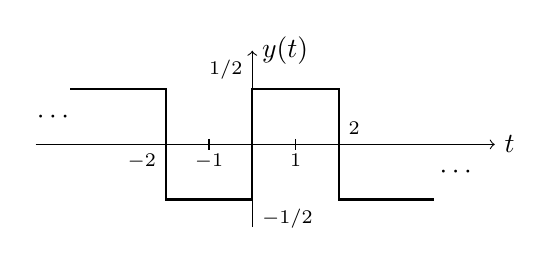
\begin{tikzpicture}[xscale=0.55, yscale=1.4]
  \draw[->] (-5,0) -- (5.6,0) node[right] {$t$};
  \draw[->] (0,-0.75) -- (0,0.85) node[right] {$y(t)$};
  \draw[thick] (-4.2,0.5) -- (-2,0.5) -- (-2,-0.5) -- (0,-0.5) -- (0,0.5) -- (2,0.5) -- (2,-0.5) -- (4.2,-0.5);
  \node at (-4.6,0.25) {$\cdots$}; \node at (4.7,-0.25) {$\cdots$};
  \node[above left] at (0,0.5) {\scriptsize $1/2$};
  \node[below right] at (0,-0.5) {\scriptsize $-1/2$};
  \foreach \x in {-2,-1,1,2} { \draw (\x,0.05) -- (\x,-0.05); }
  \node[below left] at (-2,0) {\scriptsize $-2$}; \node[below] at (-1,0) {\scriptsize $-1$};
  \node[below] at (1,0) {\scriptsize $1$}; \node[above right] at (2,0) {\scriptsize $2$};
\end{tikzpicture}
\end{minipage}\hfill
\begin{minipage}[c]{0.42\linewidth}
$y(t)$ işaretinin Fourier Serisi katsayılarını bulunuz.
\end{minipage}
\end{ornek}
\begin{cozum}
\textbf{I. yol:}
\[ y(t) = \sum_{k=-\infty}^{\infty} y_k\,e^{jk\omega_0 t}, \qquad T_0 = 4, \quad \omega_0 = \frac{2\pi}{T_0} = \frac{\pi}{2} \]
\[ y_k = \frac{1}{T_0}\int_{T_0} y(t)\,e^{-jk\omega_0 t}\,dt \]

\textbf{II. yol:}

\begin{center}
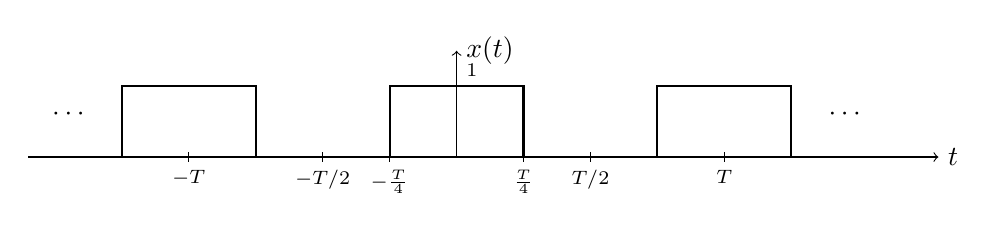
\begin{tikzpicture}[xscale=3.4, yscale=0.9]
  \draw[->] (-1.6,0) -- (1.8,0) node[right] {$t$};
  \draw[->] (0,0) -- (0,1.5) node[right] {$x(t)$};
  \foreach \c in {-1,0,1} { \draw[thick] ({\c-0.25},0) -- ({\c-0.25},1) -- ({\c+0.25},1) -- ({\c+0.25},0); }
  \node at (-1.45,0.6) {$\cdots$}; \node at (1.45,0.6) {$\cdots$};
  \node[above right] at (0,1) {\scriptsize $1$};
  \foreach \x/\l in {-1/{-T},-0.5/{-T/2},-0.25/{-\frac{T}{4}},0.25/{\frac{T}{4}},0.5/{T/2},1/{T}} { \draw (\x,0.07) -- (\x,-0.07); \node[below] at (\x,-0.05) {\scriptsize $\l$}; }
\end{tikzpicture}
\end{center}
\[ x_0 = \frac{1}{2} \qquad\qquad x_k = \frac{\sin(k\pi/2)}{\pi k}, \quad k \neq 0 \]

\[ T = 4 \ \Rightarrow\ y(t) = x(t-1) - 1/2 \]
\[ y_k = \begin{cases} x_0 - 1/2, & k = 0 \\ x_k\,e^{-jk\omega_0 t_0} = x_k\,e^{-jk\pi/2}, & k \neq 0 \end{cases} \qquad \begin{aligned} & \longleftarrow -1/2 \text{ dc offset} \\ & \longleftarrow x(t-1) \text{ zamanda kaydırma.} \end{aligned} \]
\[ y_k = \begin{cases} 0, & k = 0 \\[1mm] \dfrac{\sin(k\pi/2)\,e^{-jk\pi/2}}{k\pi}, & k \neq 0 \end{cases} \]
\end{cozum}

\begin{ornek}[(Ex)]
\sayfa{3}
\begin{center}
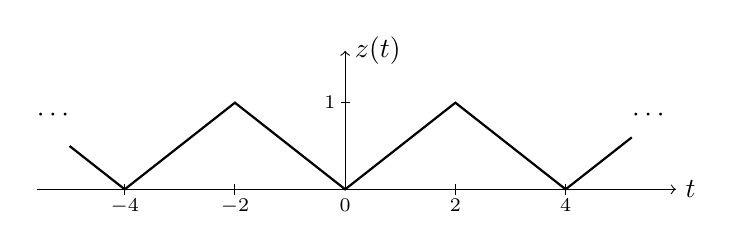
\begin{tikzpicture}[xscale=0.7, yscale=1.1]
  \draw[->] (-5.6,0) -- (6,0) node[right] {$t$};
  \draw[->] (0,0) -- (0,1.6) node[right] {$z(t)$};
  \draw[thick] (-5,0.5) -- (-4,0) -- (-2,1) -- (0,0) -- (2,1) -- (4,0) -- (5.2,0.6);
  \node at (-5.3,0.85) {$\cdots$}; \node at (5.5,0.85) {$\cdots$};
  \draw (-0.08,1) -- (0.08,1); \node[left] at (0,1) {\scriptsize $1$};
  \foreach \x in {-4,-2,2,4} { \draw (\x,0.06) -- (\x,-0.06); \node[below] at (\x,0) {\scriptsize $\x$}; }
  \node[below] at (0,0) {\scriptsize $0$};
\end{tikzpicture}
\end{center}
\end{ornek}
\begin{cozum}
\[ z(t) = |t|/2, \quad |t| < 2 \]
\[ \frac{dz(t)}{dt} = y(t) \xleftrightarrow{\ FS\ } y_k = jk\omega_0\,z_k \ \Rightarrow\ z_k = \frac{1}{jk\omega_0}\,y_k \underset{\substack{\uparrow\\ \omega_0\,=\,\pi/2}}{=} \frac{2}{jk\pi}\,y_k \]
\[ z_k = \frac{2}{j(k\pi)^2}\sin(k\pi/2)\,e^{-jk\pi/2}, \quad k \neq 0 \]
\[ z_0 = \frac{1}{T_0}\int_{T_0} z(t)\,dt = \frac{1}{2} \]
\end{cozum}

\begin{ornek}[(Ex)]
$x(t) = \displaystyle\sum_{k=-\infty}^{\infty} \delta(t - kT)$ dürtü treni olup $x_k = \dfrac{1}{T}$'dir. Aşağıda verilen işaretlerin FS katsayılarını bulunuz.
\begin{center}
\begin{tikzpicture}[xscale=1.05, yscale=0.85]
  \draw[->] (-5.4,0) -- (5.8,0) node[right] {$t$};
  \draw[->] (0,-1.4) -- (0,1.5) node[right] {$y(t)$};
  \foreach \x in {-0.8,3.2} { \draw[->, thick] (\x,0) -- (\x,1); }
  \foreach \x in {-3.2,0.8,4.8} { \draw[->, thick] (\x,0) -- (\x,-1); }
  \draw (-0.08,1) -- (0.08,1); \node[right] at (0,1.1) {\scriptsize $1$};
  \draw (-0.08,-1) -- (0.08,-1); \node[left] at (0,-1) {\scriptsize $-1$};
  \foreach \x/\l in {-4/{-T},-2/{-T/2},2/{T/2},4/{T}} { \draw (\x,0.06) -- (\x,-0.06); \node[below] at (\x,0) {\scriptsize $\l$}; }
  \node[below left] at (-0.8,0) {\scriptsize $-T_1$};
  \node[above] at (0.8,0) {\scriptsize $T_1$};
\end{tikzpicture}

\begin{tikzpicture}[xscale=1.05, yscale=0.85]
  \draw[->] (-5.6,0) -- (5.8,0) node[right] {$t$};
  \draw[->] (0,0) -- (0,1.5) node[right] {$z(t)$};
  \foreach \c in {-4,0,4} { \draw[thick] ({\c-0.8},0) -- ({\c-0.8},1) -- ({\c+0.8},1) -- ({\c+0.8},0); }
  \node at (-5.3,0.6) {$\cdots$}; \node at (5.3,0.6) {$\cdots$};
  \node[above left] at (0,1) {\scriptsize $1$};
  \foreach \x/\l in {-4/{-T},-2/{-T/2},-0.8/{-T_1},0.8/{T_1},2/{T/2},4/{T}} { \draw (\x,0.06) -- (\x,-0.06); \node[below] at (\x,0) {\scriptsize $\l$}; }
\end{tikzpicture}
\end{center}
\end{ornek}
\begin{cozum}
\[ y(t) = x(t + T_1) - x(t - T_1) \xleftrightarrow{\ FS\ } y_k = x_k\,e^{jk\omega_0 T_1} - x_k\,e^{-jk\omega_0 T_1} = \frac{1}{T}\left[e^{+jk\omega_0 T_1} - e^{-jk\omega_0 T_1}\right] \]
\[ y_k = \frac{2j}{T}\sin(k\omega_0 T_1) \]
\[ \frac{dz(t)}{dt} = y(t) \xleftrightarrow{\ FS\ } y_k = jk\omega_0\,z_k \longrightarrow z_k = \frac{1}{jk\omega_0}\,y_k = \frac{2j}{T\,jk\omega_0}\sin(k\omega_0 T_1) \]
\[ z_k = \frac{\sin(k\omega_0 T_1)}{k\pi}, \quad k \neq 0 \]
\[ z_0 = \frac{1}{T_0}\int_{T_0} z(t)\,dt = \frac{1}{T}\int_{-T_1}^{T_1} dt = \frac{2T_1}{T} \]
\end{cozum}

\begin{ornek}[(Ex)]
\begin{center}
\begin{tikzpicture}[xscale=0.62, yscale=0.85]
  \draw[->] (-8.4,0) -- (9,0) node[right] {$t$};
  \draw[->] (0,-1.6) -- (0,1.6) node[right] {$x(t)$};
  \foreach \a in {-8,-2,4} { \draw[thick] (\a,0) -- (\a,1) -- ({\a+1},1) -- ({\a+1},0); }
  \foreach \a in {-5,1,7} { \draw[thick] (\a,0) -- (\a,-1) -- ({\a+1},-1) -- ({\a+1},0); }
  \draw (-0.08,1) -- (0.08,1); \node[above left] at (0,1) {\scriptsize $1$};
  \draw (-0.08,-1) -- (0.08,-1); \node[left] at (0,-1) {\scriptsize $-1$};
  \foreach \x in {-6,-3,3,6} { \draw (\x,0.06) -- (\x,-0.06); \node[below] at (\x,0) {\scriptsize $\x$}; }
  \foreach \x in {-5,-4} { \node[above] at (\x,0) {\scriptsize $\x$}; }
  \foreach \x in {-2,-1,4,5} { \node[below] at (\x,0) {\scriptsize $\x$}; }
  \foreach \x in {1,2,7,8} { \node[above] at (\x,0) {\scriptsize $\x$}; }
  \draw[kirmizikalem, thick] (-2.1,-0.45) -- (-1.4,-0.45);
\end{tikzpicture}
\end{center}
\end{ornek}
\begin{cozum}
\[ x(t) = z(t + 3/2) - z(t - 3/2) \quad \text{ve} \quad T_1 = 1/2 \]
\begin{align*}
  x_k &= z_k\,e^{+jk\omega_0 3/2} - z_k\,e^{-jk\omega_0 3/2}, \qquad T = 6 \longrightarrow \omega_0 = \frac{2\pi}{T} = \frac{\pi}{3} \\
  x_k &= z_k\left[e^{jk\pi/2} - e^{-jk\pi/2}\right] = 2j\,z_k\sin(k\pi/2) \\
  x_k &= 2j\,\frac{1}{k\pi}\sin(k\pi/6)\,\sin(k\pi/2) \\
  x_k &= \frac{\cos(2k\pi/3) - \cos(k\pi/3)}{jk\pi}
\end{align*}
\end{cozum}

\section{Sürekli Zamanlı LTI sistemlerin Periyodik İşaretlere Cevabı}
\sayfa{4}
\begin{center}
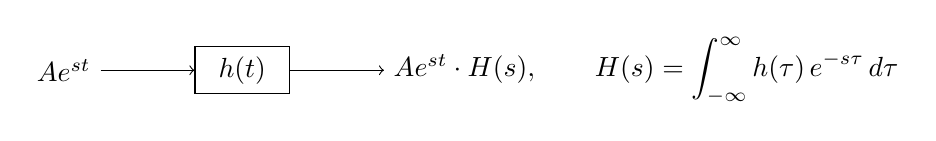
\begin{tikzpicture}
  \node[draw, minimum width=1.2cm, minimum height=0.6cm] (H) at (0,0) {$h(t)$};
  \draw[->] (-1.8,0) node[left] {$A e^{st}$} -- (H.west);
  \draw[->] (H.east) -- (1.8,0) node[right] {$A e^{st}\cdot H(s), \qquad H(s) = \displaystyle\int_{-\infty}^{\infty} h(\tau)\,e^{-s\tau}\,d\tau$};
\end{tikzpicture}
\end{center}
$\Rightarrow$ Bir sistemin çıktısı, girdinin bir sabit ile çarpımı ise, o girdi işaretine sistemin özfonksiyonu (eigenfunction), ilgili sabite (genlik çarpanına) özdeğeri (eigenvalue) denir.
\begin{gather*}
  y(t) = x(t) \ast h(t) = \int_{-\infty}^{\infty} x(\tau)\,h(t-\tau)\,d\tau = \int_{-\infty}^{\infty} h(\tau)\,x(t-\tau)\,d\tau \\
  y(t) = \int_{-\infty}^{\infty} h(\tau)\,A e^{s(t-\tau)}\,d\tau = A e^{st}\underbrace{\int_{-\infty}^{\infty} h(\tau)\,e^{-s\tau}\,d\tau}_{\triangleq\,H(s)} = A e^{st} H(s) \longrightarrow \begin{aligned}[t] & A e^{st}: \text{özfonksiyon} \\ & \hookrightarrow H(s): \text{özdeğer} \end{aligned}
\end{gather*}
$\Rightarrow$ $s = j\omega$
\begin{center}
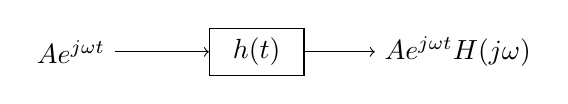
\begin{tikzpicture}
  \node[draw, minimum width=1.2cm, minimum height=0.6cm] (H) at (0,0) {$h(t)$};
  \draw[->] (-1.8,0) node[left] {$A e^{j\omega t}$} -- (H.west);
  \draw[->] (H.east) -- (1.5,0) node[right] {$A e^{j\omega t} H(j\omega)$};
\end{tikzpicture}
\end{center}
\[ H(j\omega) = \int_{-\infty}^{\infty} h(t)\,e^{-j\omega t}\,dt \ : \ \text{Frequency Response (Frekans cevabı)} \]
\begin{center}
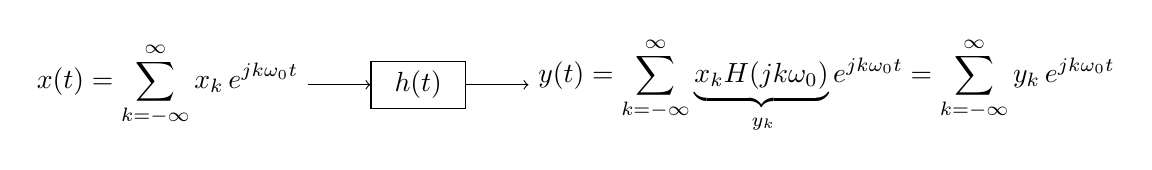
\begin{tikzpicture}
  \node[draw, minimum width=1.2cm, minimum height=0.6cm] (H) at (0,0) {$h(t)$};
  \draw[->] (-1.4,0) node[left] {$x(t) = \displaystyle\sum_{k=-\infty}^{\infty} x_k\,e^{jk\omega_0 t}$} -- (H.west);
  \draw[->] (H.east) -- (1.4,0) node[right] {$y(t) = \displaystyle\sum_{k=-\infty}^{\infty} \underbrace{x_k H(jk\omega_0)}_{\triangleq\,y_k} e^{jk\omega_0 t} = \sum_{k=-\infty}^{\infty} y_k\,e^{jk\omega_0 t}$};
\end{tikzpicture}
\end{center}
Bir LTI sistemin girişinde hangi frekans bileşenleri varsa çıkışında da o frekans bileşenleri vardır.

\begin{ornek}[(Ex)]
$x(t) = \displaystyle\sum_{k=-3}^{3} x_k\,e^{jk2\pi t}$, \quad $x_0 = 1$, \ $x_1 = x_{-1} = \dfrac{1}{4}$, \ $x_2 = x_{-2} = \dfrac{1}{2}$, \ $x_3 = x_{-3} = \dfrac{1}{3}$
\begin{enumerate}[label=\alph*)]
  \item $x(t) = ?$
  \item $h(t) = e^{-t}u(t)$ ise $y(t) = ?$
\end{enumerate}
\end{ornek}
\begin{cozum}
\textbf{a)}
\begin{gather*}
  x(t) = 1 + \frac{1}{4}\left[e^{j2\pi t} + e^{-j2\pi t}\right] + \frac{1}{2}\left[e^{j4\pi t} + e^{-j4\pi t}\right] + \frac{1}{3}\left[e^{j6\pi t} + e^{-j6\pi t}\right] \\
  x(t) = 1 + \frac{1}{2}\cos(2\pi t) + \cos(4\pi t) + \frac{2}{3}\cos(6\pi t)
\end{gather*}
\textbf{b)}
\[ y(t) = \sum_{k=-\infty}^{\infty} y_k\,e^{jk\omega_0 t} = \sum_{k=-\infty}^{\infty} x_k H(jk\omega_0)\,e^{jk\omega_0 t}, \qquad \omega_0 = 2\pi \]
\[ H(j\omega) = \int_{-\infty}^{\infty} h(t)\,e^{-j\omega t}\,dt = \int_{0}^{\infty} e^{-t}\cdot e^{-j\omega t}\,dt = \int_{0}^{\infty} e^{-(1+j\omega)t}\,dt = \frac{e^{-(1+j\omega)t}}{-(1+j\omega)}\Bigg|_{0}^{\infty} = \frac{1}{1+j\omega} \]
\begin{align*}
  y_k &= x_k H(jk\omega_0) = x_k H(jk2\pi) \\
  y_0 &= x_0 = 1 \\
  y_1 &= x_1 H(j2\pi) = \frac{1}{4}\left(\frac{1}{1+j2\pi}\right) \\
  y_{-1} &= x_{-1} H(-j2\pi) = \frac{1}{4}\left(\frac{1}{1-j2\pi}\right)
\end{align*}
\[ y_2 = \frac{1}{2}\left(\frac{1}{1+j4\pi}\right) \qquad y_{-2} = \frac{1}{2}\left(\frac{1}{1-j4\pi}\right) \qquad y_3 = \frac{1}{3}\left(\frac{1}{1+j6\pi}\right) \qquad y_{-3} = \frac{1}{3}\left(\frac{1}{1-j6\pi}\right) \]
\end{cozum}

\begin{ornek}[(Ex)]
\sayfa{5}
$x(t) = \cos(2t + \pi/4)$, \quad $x_k = ?$ \quad $P_x = ?$
\end{ornek}
\begin{cozum}
\[ x(t) = \frac{1}{2}\left[e^{j(2t + \pi/4)} + e^{-j(2t + \pi/4)}\right] = \frac{1}{2}e^{j\pi/4}\cdot e^{j2t} + \frac{1}{2}e^{-j\pi/4}\cdot e^{-j2t}, \qquad \omega_0 = 2 \rightarrow T = \frac{2\pi}{\omega_0} = \pi \]
\[ x_1 = \frac{1}{2}e^{j\pi/4} \qquad x_{-1} = \frac{1}{2}e^{-j\pi/4} \]
\[ P_x = \frac{1}{T}\int_{T} |x(t)|^2\,dt = \sum_{k=-\infty}^{\infty} |x_k|^2 = \left(\frac{1}{2}\right)^2\cdot 2 = \frac{1}{2} \]
\end{cozum}

\begin{ornek}[(Ex)]
$x_k = \begin{cases} jk, & |k| \leq 3 \\ 0, & \text{dışında} \end{cases}$ \quad ise \ $x(t) = ?$
\end{ornek}
\begin{cozum}
\[ x(t) = \sum_{k=-3}^{3} x_k\,e^{jk\omega_0 t} \quad \longleftarrow \ \begin{aligned}[t] & x_0 = 0 \\ & x_1 = j \qquad x_{-1} = -j \\ & x_2 = 2j \quad\ \ x_{-2} = -2j \\ & x_3 = 3j \quad\ \ x_{-3} = -3j \end{aligned} \]
\begin{gather*}
  x(t) = j\left[e^{j\omega_0 t} - e^{-j\omega_0 t}\right] + 2j\left[e^{j2\omega_0 t} - e^{-j2\omega_0 t}\right] + 3j\left[e^{j3\omega_0 t} - e^{-j3\omega_0 t}\right] \\
  x(t) = -2\sin\omega_0 t - 4\sin(2\omega_0 t) - 8\sin(3\omega_0 t) \quad \text{\footnotemark}
\end{gather*}
\end{cozum}
\footnotetext{Claude notu: muhtemelen $-6\sin(3\omega_0 t)$ olmalı ($3j\cdot 2j\sin 3\omega_0 t = -6\sin 3\omega_0 t$).}

\begin{ornek}[(Ex)]
$H(j\omega) = \begin{cases} 1, & |\omega| \leq 100 \\ 0, & |\omega| > 100 \end{cases}$ \qquad
\begin{minipage}[t]{0.55\linewidth}
$x(t)$'nin periyodu $T = \pi/6$\\
$y(t) = x(t)$ olması için hangi $k$ değerleri için $x_k = 0$ olmalıdır.
\end{minipage}
\end{ornek}
\begin{cozum}
\[ y(t) = \sum_{k=-\infty}^{\infty} y_k\,e^{jk\omega_0 t} = \sum_{k=-\infty}^{\infty} x_k H(jk\omega_0)\,e^{jk\omega_0 t} \]
\[ \left.\begin{aligned} & |k\omega_0| \leq 100 \\ & \omega_0 = \frac{2\pi}{T} = \frac{2\pi}{\pi/6} = 12 \end{aligned}\ \right\}\ |k| \leq \frac{100}{12} = 8.3 \ \rightarrow\ |k| \leq 8 \ \rightarrow\ |k| > 8 \]
\end{cozum}

\begin{ornek}[(Ex) \textcolor{gtufosfor-pembe}{$\bigstar$}]
Bir $x(t)$ işareti, aşağıda listelenen özellikleri ile ($\mp$ işareti dışında) belirlenebilir mi?
\begin{enumerate}[label=\arabic*.]
  \item Reeldir.
  \item $T_0 = 4$ periyodu ile periyodiktir ve FS katsayıları $x_k$'dır.
  \item $x_k = 0$, $|k| > 1$.
  \item FS katsayıları $y_k = e^{-jk\pi/2}\cdot x_{-k}$ olan $y(t)$ sinyali tektir.
  \item $\dfrac{1}{4}\displaystyle\int_{4} |x(t)|^2\,dt = 1/2$.
\end{enumerate}
\end{ornek}
\begin{cozum}
\textbf{2.} \ $T_0 = 4 \longrightarrow \omega_0 = \dfrac{2\pi}{T_0} = \dfrac{\pi}{2}$

\textbf{3.} \ $x_k = 0, \ |k| > 1 \longrightarrow x(t) = \displaystyle\sum_{k=-1}^{1} x_k\,e^{jk\omega_0 t} = x_0 + x_1\,e^{jk\pi t/2} + x_{-1}\,e^{-jk\pi t/2}$

\textbf{1.} \ $x(t)$ Reel $\longrightarrow x(t) = x^{*}(t) \Rightarrow x_k = x_{-k}^{*}$ ve $x_0$ Reel
\[ x(t) = x_0 + x_1\,e^{jk\omega_0 t} + \left(x_1\,e^{jk\omega_0 t}\right)^{*} = x_0 + 2\,\mathrm{Re}\left\{x_1\,e^{jk\pi t/2}\right\} \]

\textbf{4.} \ $y_k = e^{-jk\pi/2}\cdot x_{-k} \longrightarrow x(t) \xleftrightarrow{\ FS\ } x_k$ ise \ $x(-t) \xleftrightarrow{\ FS\ } x_{-k}$
\[ x(t - t_0) \xleftrightarrow{\ FS\ } x_k\,e^{-jk\omega_0 t_0} \]
\[ y(t) = x(-t+1) \text{ reel ve tektir.} \longrightarrow y_k \text{ sanal ve tek} \longrightarrow \begin{aligned}[t] & y_0 = 0 \\ & \hookrightarrow y_k = -y_{-k} \quad (y_1 = -y_{-1}) \end{aligned} \]

\textbf{5.}
\sayfa{6}
\[ \frac{1}{4}\int_{4} |x(t)|^2\,dt = \sum_{k=-\infty}^{\infty} |x_k|^2 = \sum_{k} |y_k|^2 = |y_0|^2 + |y_1|^2 + |y_{-1}|^2 \]
\[ 2|y_1|^2 = \frac{1}{2} \longrightarrow |y_1| = \frac{1}{2} \]
$y_k$ sanal olacağından \ $y_1 = \mp j/2$
\[ x_{-k} = y_k\,e^{jk\pi/2}\ \begin{cases}
  \longrightarrow x_0 = 0 \\[2mm]
  \longrightarrow y_1 = j/2 \Rightarrow \left.\begin{aligned} & x_{-1} = \frac{j}{2}\,e^{j\pi/2} = \frac{-1}{2} \\ & x_{-1}^{*} = x_1 = \frac{-1}{2} \end{aligned}\ \right\}\ x(t) = 2\,\mathrm{Re}\left\{\frac{-1}{2}\,e^{j\pi t/2}\right\} = -\cos(\pi t/2) \\[6mm]
  \longrightarrow y_1 = -j/2 \Rightarrow x_{-1} = \dfrac{1}{2} = x_1 \longrightarrow x(t) = \cos(\pi t/2)
\end{cases} \]
\end{cozum}

\end{document}
